\documentclass[preprint,12pt,aps,pra,showkeys,amsmath,amssymb,superscriptaddress,floatfix]{revtex4-2}
\usepackage[T1]{fontenc}
\usepackage[utf8]{inputenc}
\usepackage{amsmath,amssymb,amsthm,mathtools,mathrsfs}
\usepackage{microtype,booktabs,enumitem}
\usepackage{xcolor,tikz,etoolbox}
\usepackage[skins,breakable]{tcolorbox}
\usepackage{needspace}
% Keep diagram geometry independent of REVTeX preprint body spacing.
\AtBeginEnvironment{tikzpicture}{\linespread{1}\selectfont}
\usetikzlibrary{arrows.meta,positioning,calc,fit,decorations.pathreplacing}
\usepackage{graphicx}
\usepackage{hyperref}

\definecolor{MMBlue}{RGB}{0,82,155}
\definecolor{MMOrange}{RGB}{200,80,0}
\tikzset{
 mmnode/.style={draw=MMBlue,rounded corners=2pt,fill=MMBlue!4,align=left,execute at begin node={\raggedright},text width=5cm,font=\fontsize{10}{12}\selectfont,inner sep=6pt},
 mmimport/.style={mmnode,draw=black!65,fill=black!4},
 mmcandidate/.style={mmnode,draw=MMOrange,dashed,fill=MMOrange!5},
 mmrejected/.style={mmnode,draw=black,densely dotted,fill=black!8},
 mmproof/.style={->,thick,MMBlue},
 mmflow/.style={->,semithick,black!70},
 mmrepair/.style={->,dashed,thick,MMOrange},
 mmcandidatearrow/.style={->,dashed,semithick,MMOrange},
 mmnote/.style={font=\scriptsize,fill=white,inner sep=2pt,align=center}}

\usepackage[section]{placeins}
\setlength{\emergencystretch}{3em}
\setlist{itemsep=3pt,topsep=4pt}
\newtheorem{theorem}{Theorem}[section]
\newtheorem{proposition}[theorem]{Proposition}
\newtheorem{lemma}[theorem]{Lemma}
\newtheorem{corollary}[theorem]{Corollary}
\theoremstyle{definition}
\newtheorem{definition}[theorem]{Definition}
\newtheorem{example}[theorem]{Example}
\theoremstyle{remark}
\newtheorem{remark}[theorem]{Remark}
% Avoid isolated statement headings and single-line paragraph fragments.
\BeforeBeginEnvironment{theorem}{\Needspace{6\baselineskip}}
\BeforeBeginEnvironment{definition}{\Needspace{5\baselineskip}}
\BeforeBeginEnvironment{proposition}{\Needspace{5\baselineskip}}
\BeforeBeginEnvironment{lemma}{\Needspace{5\baselineskip}}
\BeforeBeginEnvironment{corollary}{\Needspace{5\baselineskip}}
\clubpenalty=5000
\widowpenalty=5000
\newcommand{\R}{\mathbb R}\newcommand{\Z}{\mathbb Z}\newcommand{\N}{\mathbb N}
\newcommand{\Pa}{\operatorname{Pa}}\newcommand{\Desc}{\operatorname{Desc}}
\newcommand{\cl}{\operatorname{cl}}\newcommand{\cost}{\operatorname{cost}}
\newcommand{\status}{\operatorname{status}}
% Faculty cards: a visual rail groups the five faculties within one agent.
% The rail has no arrowhead and does not represent a proof dependency.
\newcommand{\mmfacultybadge}[1]{%
 \node[circle,draw=MMBlue,line width=1pt,fill=white,
 minimum size=7mm,inner sep=0pt,font=\sffamily\small\bfseries,text=MMBlue]
 at ([xshift=15pt,yshift=-15pt]frame.north west) {#1};}
\newcommand{\mmfacultyrail}{%
 \draw[MMBlue!80,line width=1pt]
 ([xshift=15pt,yshift=2pt]frame.north west)--
 ([xshift=15pt,yshift=-2pt]frame.south west);}
\newtcolorbox{mmfacultybox}[2]{enhanced,breakable,
 colback=MMBlue!4,colframe=MMBlue!4,boxrule=0pt,arc=3pt,
 left=39pt,right=9pt,top=4pt,bottom=4pt,
 before skip=2pt,after skip=2pt,
 fontupper=\small\linespread{1.1}\selectfont,
 overlay unbroken={\mmfacultyrail\mmfacultybadge{#1}},
 overlay first={\mmfacultyrail\mmfacultybadge{#1}},
 overlay middle={\mmfacultyrail},overlay last={\mmfacultyrail}}
\newcommand{\mmfaculty}[3]{%
 \begin{mmfacultybox}{#1}{#2}
 {\sffamily\bfseries\color{MMBlue}#2}\par\smallskip #3
 \end{mmfacultybox}}
\newcommand{\agent}[9]{%
 \Needspace{8\baselineskip}
 \subsubsection{#1}
 \noindent\textbf{Object.} #2\par
 \noindent\textbf{Role.} #3\par\smallskip
 \mmfaculty{E}{Ego}{#4}
 \mmfaculty{M}{Memory}{#5}
 \mmfaculty{I}{Intellect}{#6}
 \mmfaculty{S}{Sense}{#7}
 \mmfaculty{A}{Action}{#8}
 \smallskip\noindent #9\par}

\usepackage{longtable,array,calc}
\providecommand{\tightlist}{\setlength{\itemsep}{2pt}\setlength{\parskip}{0pt}}
\makeatletter
\def\frontmatter@abstract@produce{\par\addvspace{\frontmatter@preabstractspace}%
\begingroup\prep@absbox\unvbox\absbox\post@absbox\endgroup
\addvspace{\frontmatter@postabstractspace}}
\makeatother
\newcommand{\field}[2]{\par\smallskip\noindent\textbf{#1.} #2\par}
\setlength{\emergencystretch}{5em}
\AtBeginEnvironment{verbatim}{\small\linespread{1.0}\selectfont}


\hypersetup{colorlinks=true,linkcolor=MMBlue,urlcolor=MMBlue,pdfauthor={Dibakar Sigdel}}

\begin{document}

\title{Tychonoff's Theorem for Compact Hausdorff Spaces\\[4pt]\large An End-to-End Meta-Math Walkthrough}

\author{Dibakar Sigdel}

\affiliation{Mindverse Computing LLC, Lynnwood, WA 98087, USA}

\date{October 2026}

\begin{abstract}

A complete authored walkthrough of tychonoff's theorem for compact
hausdorff spaces, with explicit mathematical contracts, local
verification gates, and reusable exports. The report presents the target
theorem, declared imports, a dependency graph, five-faculty node
contracts, a continuous proof, a worked example, and a hypothesis-repair
audit. It is an authored mathematical exposition, not a deployed-agent
transcript or a formal proof-assistant certificate.

\end{abstract}\maketitle\linespread{1.12}\selectfont

\noindent\textbf{GT-05 / General Topology / Report v1}

\section{Target and import contract}

\begin{theorem}

Working in ZFC, prove that an arbitrary product \(\prod_{i\in I}X_i\) of
nonempty compact Hausdorff spaces is compact and Hausdorff in the
product topology.

\end{theorem}

\subsection{Foundations and permitted imports}

Work in ZFC. Import the ultrafilter extension principle: every proper
filter extends to an ultrafilter. Import the compactness criterion: a
space is compact iff every ultrafilter on it converges to some point.
This follows by applying the finite-intersection property to closed sets
and, conversely, extending a hypothetical cover-with-no-finite-subcover
complement filter. In a Hausdorff space an ultrafilter has at most one
limit. The nonempty product is available by choice.

\clearpage\section{Node interaction workflow}

\begin{center}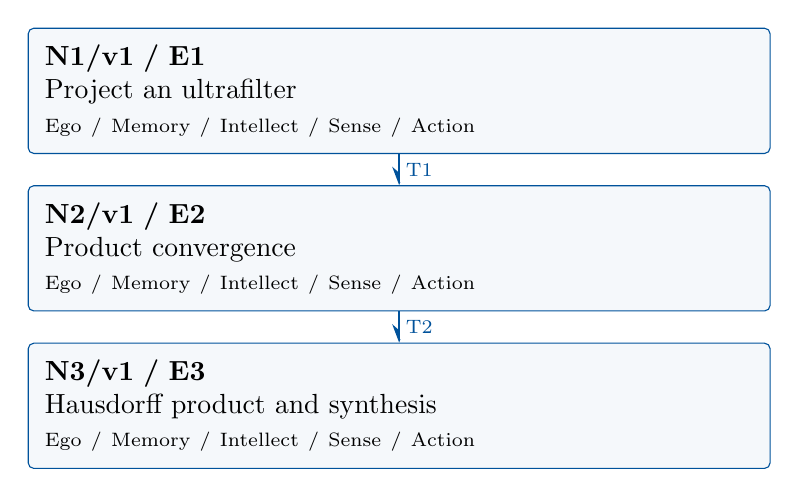
\begin{tikzpicture}[>=Stealth,x=1cm,y=1cm]

\node[mmnode,text width=9cm,minimum height=1.25cm] (N1) at (0,0.0) {\textbf{N1/v1 / E1}\\Project an ultrafilter\\{\scriptsize Ego / Memory / Intellect / Sense / Action}};

\node[mmnode,text width=9cm,minimum height=1.25cm] (N2) at (0,-2.0) {\textbf{N2/v1 / E2}\\Product convergence\\{\scriptsize Ego / Memory / Intellect / Sense / Action}};

\node[mmnode,text width=9cm,minimum height=1.25cm] (N3) at (0,-4.0) {\textbf{N3/v1 / E3}\\Hausdorff product and synthesis\\{\scriptsize Ego / Memory / Intellect / Sense / Action}};

\draw[mmproof] (N1.south) -- node[mmnote,right] {T1} (N2.north);

\draw[mmproof] (N2.south) -- node[mmnote,right] {T2} (N3.north);

\end{tikzpicture}\end{center}

Each box is one mathematical agent containing all five faculties. Blue
arrows carry the versioned exports listed below. The layout gives a
reading order; only drawn arrows assert dependencies. Diagnostic repair
is separate from the proof DAG.

\subsection{Versioned evidence-transfer ledger}

\begingroup\small\linespread{1.05}\selectfont

\Needspace{5\baselineskip}\field{T1: N1/E1/v1 to N2}{A coordinate limit tuple for every ultrafilter on the product.}

\field{Receiving activity}{N2: Product convergence}

\field{Compatibility}{Use the same mathematical objects and hypotheses as the source export.
Receiving contract: All coordinate limits; prior exports E1/v1}

\Needspace{5\baselineskip}\field{T2: N2/E2/v1 to N3}{Every ultrafilter on X converges; X is compact.}

\field{Receiving activity}{N3: Hausdorff product and synthesis}

\field{Compatibility}{Use the same mathematical objects and hypotheses as the source export.
Receiving contract: Distinct product points; prior exports E2/v1}

\endgroup

\clearpage\section{Agent roles and five-faculty activities}\begingroup\small\linespread{1.05}\selectfont\setlist{itemsep=1pt,topsep=2pt}

\subsection{N1/v1: Project an ultrafilter}

\field{Object and role}{Push the filter through each coordinate map.}

\field{Inputs}{\(X=\prod X_i\) and an ultrafilterU on X; foundational imports stated in
§1}

\mmfaculty{E}{Ego}{Own E1/v1: A coordinate limit tuple for every ultrafilter on the
product.}

\mmfaculty{M}{Memory}{Retain \(X=\prod X_i\) and an ultrafilterU on X; foundational imports
stated in §1; keep their assumptions and versions attached.}

\mmfaculty{I}{Intellect}{Push the filter through each coordinate map.}

\mmfaculty{S}{Sense}{Convergence is an ultrafilter notion; no sequential compactness shortcut
is used.}

\mmfaculty{A}{Action}{Carry out the numbered deductions and publish E1/v1 together with its
hypotheses and proof location.}

\smallskip\noindent\textbf{Numbered mathematical activities}

\begin{enumerate}[label=N1.\arabic*,leftmargin=3.4em]

\item For eachi define \(U_i=\{A\subset X_i:\pi _i^{-1}(A)\in U\}\).

\item Inverse images preserve complements, inclusions, and finite
intersections, so \(U_i\) is a proper ultrafilter: for each A exactly
one of A or its complement belongs.

\item Compactness of \(X_i\) gives a limit \(x_i\); Hausdorffness makes it
unique.

\item The tuple \(x=(x_i)\) is a point of X.

\item If I is empty the product is a singleton and the result is immediate.

\end{enumerate}

\field{Export E1/v1}{A coordinate limit tuple for every ultrafilter on the product.}

\field{Acceptance gate}{Convergence is an ultrafilter notion; no sequential compactness shortcut
is used. Publish only after checking every displayed deduction.}

\field{Targeted repair}{If the check fails, revise N1: Convergence is an ultrafilter notion; no
sequential compactness shortcut is used. Recheck dependent nodes N2, N3.}

\clearpage

\subsection{N2/v1: Product convergence}

\field{Object and role}{Check only finitely many coordinate constraints at a time.}

\field{Inputs}{All coordinate limits; prior exports E1/v1}

\mmfaculty{E}{Ego}{Own E2/v1: Every ultrafilter on X converges; X is compact.}

\mmfaculty{M}{Memory}{Retain All coordinate limits; prior exports E1/v1; keep their
assumptions and versions attached.}

\mmfaculty{I}{Intellect}{Check only finitely many coordinate constraints at a time.}

\mmfaculty{S}{Sense}{A filter need not be closed under infinitely many intersections.}

\mmfaculty{A}{Action}{Carry out the numbered deductions and publish E2/v1 together with its
hypotheses and proof location.}

\smallskip\noindent\textbf{Numbered mathematical activities}

\begin{enumerate}[label=N2.\arabic*,leftmargin=3.4em]

\item A basic neighborhood ofx has form \(B=\cap _{i\in F}\pi _i^{-1}(V_i)\)
with F finite and \(V_i\) a neighborhood of \(x_i\).

\item Since \(U_i\to x_i\), every \(V_i\) belongs to \(U_i\); hence each
inverse image belongs to U.

\item A filter is closed under finite intersections, so \(B\in U\).

\item Any neighborhood contains such aB and is therefore in U.

\item Thus U converges tox.

\item The imported criterion proves X compact.

\end{enumerate}

\field{Export E2/v1}{Every ultrafilter on X converges; X is compact.}

\field{Acceptance gate}{A filter need not be closed under infinitely many intersections. Publish
only after checking every displayed deduction.}

\field{Targeted repair}{If the check fails, revise N2: A filter need not be closed under
infinitely many intersections. Recheck dependent nodes N3.}

\clearpage

\subsection{N3/v1: Hausdorff product and synthesis}

\field{Object and role}{Separate using one differing coordinate.}

\field{Inputs}{Distinct product points; prior exports E2/v1}

\mmfaculty{E}{Ego}{Own E3/v1: The product is compact and Hausdorff.}

\mmfaculty{M}{Memory}{Retain Distinct product points; prior exports E2/v1; keep their
assumptions and versions attached.}

\mmfaculty{I}{Intellect}{Separate using one differing coordinate.}

\mmfaculty{S}{Sense}{The topology is the product topology; the box topology has different
basic neighborhoods.}

\mmfaculty{A}{Action}{Carry out the numbered deductions and publish E3/v1 together with its
hypotheses and proof location.}

\smallskip\noindent\textbf{Numbered mathematical activities}

\begin{enumerate}[label=N3.\arabic*,leftmargin=3.4em]

\item If \(x\ne y\), some coordinatei has \(x_i\ne y_i\).

\item Hausdorffness of \(X_i\) gives disjoint open neighborhoodsV,W.

\item Their projection inverse images are disjoint open neighborhoods ofx,y in
X.

\item Hence X is Hausdorff.

\item Together with node2 this proves the arbitrary-product theorem under its
stated foundations.

\end{enumerate}

\field{Export E3/v1}{The product is compact and Hausdorff.}

\field{Acceptance gate}{The topology is the product topology; the box topology has different
basic neighborhoods. Publish only after checking every displayed
deduction.}

\field{Targeted repair}{If the check fails, revise N3: The topology is the product topology; the
box topology has different basic neighborhoods. Withhold this terminal
result until its gate passes.}

\endgroup\clearpage\section{Continuous mathematical proof}\label{sec:proof}

Read these steps in order as one proof; the diagram is optional.
Numbered activities identify the specific constructions and deductions
owned by each node.

\subsection{§4.N1 --- Project an
ultrafilter}\label{n1-project-an-ultrafilter}

Let \(X=\prod_i X_i\) and choose an arbitrary ultrafilter \(\mathcal U\)
on \(X\).

\begin{enumerate}
\def\labelenumi{\arabic{enumi}.}
\item
  For eachi define \(U_i=\{A\subset X_i:\pi _i^{-1}(A)\in U\}\).
\item
  Inverse images preserve complements, inclusions, and finite
  intersections, so \(U_i\) is a proper ultrafilter: for each A exactly
  one of A or its complement belongs.
\item
  Compactness of \(X_i\) gives a limit \(x_i\); Hausdorffness makes it
  unique.
\item
  The tuple \(x=(x_i)\) is a point of X.
\item
  If I is empty the product is a singleton and the result is immediate.
\end{enumerate}

\subsection{§4.N2 --- Product convergence}\label{n2-product-convergence}

\begin{enumerate}
\def\labelenumi{\arabic{enumi}.}
\item
  A basic neighborhood ofx has form \(B=\cap _{i\in F}\pi _i^{-1}(V_i)\)
  with F finite and \(V_i\) a neighborhood of \(x_i\).
\item
  Since \(U_i\to x_i\), every \(V_i\) belongs to \(U_i\); hence each
  inverse image belongs to U.
\item
  A filter is closed under finite intersections, so \(B\in U\).
\item
  Any neighborhood contains such aB and is therefore in U.
\item
  Thus U converges tox.
\item
  The imported criterion proves X compact.
\end{enumerate}

\subsection{§4.N3 --- Hausdorff product and
synthesis}\label{n3-hausdorff-product-and-synthesis}

\begin{enumerate}
\def\labelenumi{\arabic{enumi}.}
\item
  If \(x\ne y\), some coordinatei has \(x_i\ne y_i\).
\item
  Hausdorffness of \(X_i\) gives disjoint open neighborhoodsV,W.
\item
  Their projection inverse images are disjoint open neighborhoods ofx,y
  in X.
\item
  Hence X is Hausdorff.
\item
  Together with node2 this proves the arbitrary-product theorem under
  its stated foundations.
\end{enumerate}

\hfill$\square$

\section{Worked orchestration}

For \(X=[0,1]^I\) with an arbitrarily large index set, a basic open
neighborhood specifies finitely many coordinates. The ultrafilter proof
treats any I uniformly; it never orders its elements into a sequence.
For \(I=\{1,2\}\) it reproduces compactness of the square.

\subsection{Boundary and hypothesis audit}

In the countable box \(product[0,1]^N\), points \(x^{(n)}\) with firstn
coordinates0 and all others1 have no convergent subsequence: every
coordinate forces any putative subsequence limit to be0, while the box
neighborhood \(\prod [0,1/2\)) excludes every term. A compact Hausdorff
space makes each infinite set have an accumulation point, and this
particular set has none: 0 has the displayed box neighborhood excluding
every term; for any other point x, choose a coordinate k with \(x_k>0\)
and a coordinate neighborhood avoiding 0, which excludes all terms with
\(n\ge k\). The remaining finite terms can be excluded individually by
Hausdorff neighborhoods, so x is not an accumulation point either. Thus
the box product is not compact. Sense keeps the finite-coordinate
product topology rather than substituting infinite intersections.

\section{Illustrative failure and repair}

The following is an authored diagnostic scenario. Changed assumptions
define a new contract; they do not retroactively prove the original
statement.

\subsection{Failure and correction}
This is an authored teaching trace, not a recorded agent run.

\begin{enumerate}
\def\labelenumi{\arabic{enumi}.}
\tightlist
\item
  \textbf{Ego \(\to\) Memory:} register the §1 theorem, imports, and
  requested exports before beginning the proof.
\item
  \textbf{Intellect \(\to\) Action:} choose the bridges in §3 and carry
  out the numbered activities in §4; transmit only established E-exports
  along the §2 DAG.
\item
  \textbf{Sense \(\to\) responsible node:} test the specific
  boundary/failure in §5 and the node's individual audit. A failing
  candidate is withheld; downstream nodes may not use it.
\item
  \textbf{Memory + Intellect:} identify whether the error is an omitted
  condition, an invalid inference, or an attempted extension beyond the
  theorem. Restore the exact contract or explicitly state a different
  one.
\item
  \textbf{Action:} redo the affected mathematical activity using the
  repaired condition or inference. Recheck consuming nodes, rather than
  feeding their conclusions back as premises.
\item
  \textbf{Ego:} publish only the supported export with its assumptions
  and proof location. A hypothetical revised export is v2; the written
  proof here is the v1 exposition, not a claim that this repair was
  executed.
\end{enumerate}

\subsection{Hypothesis boundary}
In the countable box \(product[0,1]^N\), points \(x^{(n)}\) with firstn
coordinates0 and all others1 have no convergent subsequence: every
coordinate forces any putative subsequence limit to be0, while the box
neighborhood \(\prod [0,1/2\)) excludes every term. A compact Hausdorff
space makes each infinite set have an accumulation point, and this
particular set has none: 0 has the displayed box neighborhood excluding
every term; for any other point x, choose a coordinate k with \(x_k>0\)
and a coordinate neighborhood avoiding 0, which excludes all terms with
\(n\ge k\). The remaining finite terms can be excluded individually by
Hausdorff neighborhoods, so x is not an accumulation point either. Thus
the box product is not compact. Sense keeps the finite-coordinate
product topology rather than substituting infinite intersections.

\subsection{Version and recheck}
Treat any changed assumption as a new contract. Recheck the revised
export and all of its descendants. A backward diagnostic never
establishes an earlier theorem. This is an authored teaching trace, not
an execution log.

\par\medskip\begingroup\small\linespread{1.0}\selectfont\noindent\textbf{Provenance.} This authored proof is complete relative to its declared imports. Reuse
each export with its assumptions, proof, and version. The original
Markdown remains available for comparison.
\par\endgroup

\par\smallskip\begingroup\small\linespread{1.0}\selectfont\noindent\textbf{Further reading.} \begin{itemize}
\tightlist
\item
  \href{https://ocw.mit.edu/courses/18-901-introduction-to-topology-fall-2004/pages/lecture-notes/}{MIT
  Introduction to Topology: separation, Urysohn, and Tychonoff
  material}.
\end{itemize}\par\endgroup

\end{document}
